%!TEX root = origin_elements_lecture_notes.tex

\chapter{Galactic Chemical Evolution}

Finally, after having discussed many formation scenarios for elements in the universe, it is time to hang it all together to look at how the solar composition came together after roughly 9\,Ga of Milky Way evolution. The evolution of all elements and isotopes in the galaxy is generally referred to as \acf{gce}. Some authors also prefer the term ``galactic archeology'', since it has many common points with regular archeology. In the \ac{gce} sense, the evolution tracks of the individual elements and their abundances are the galactic fossils that can be used to decipher the origin of the material we are all made of.

\section{The Basic Ingredients}

The four basic ingredients necessary to model \ac{gce} are the initial conditions, the stellar birthrate function, the nucleosynthesis yields that get recycled back into the universe, and gas infall and outflow rates from the galaxy. With all of these ingredients provided, we can describe the chemical abundance of an element $X_i$ over time. At any given time and location, the abundance $X_i$ can be expressed as the mass fraction of the total amount of gas, i.e.,
\begin{equation}
    X_i = \frac{M_i}{M_\mathrm{gas}}.
\end{equation}
According to this definition, we can write $\sum_i X_i = 1$. As introduced in Chapter~\ref{ch:solar_system_abundances}, the abundances of hydrogen, helium, and all other elements are usually written as $X$, $Y$, and $Z$, respectively.

\subsection{Initial Conditions}

Depending on where a given \ac{gce} model starts, an initial composition must be assumed. This composition can be the primordial abundance, i.e., the elements that formed in the Big Bang, or can be some composition enriched by previous pre-galactic stellar generations. Modern chemodynamical models (see below) generally start with the Big Bang and model the formation and evolution of the whole galaxy up to the present day. In addition to the composition we need to define if the galaxy to be modeled is a closed system (closed box approach) or if gas infall and outflow takes place. Gas inflow could, e.g., happen when gas from the galactic halo is accreted onto the disk, outflow on the other hand would be similar to galactic winds.


\subsection{Birthrate Function}

The birthrate function $B(m,t)$ describes how many stars in the mass interval between $m$ and $m+dm$ form in a given time interval between time $t$ and $t+dt$. It can be written as
\begin{equation}
    B(m,t) = \psi(t) \phi(m).
\end{equation}
Here, the quantity $\psi(t)$ is the \acf{sfr}, which is equal to the rate at which interstellar gas is turned into stars per unit time. The quantity $\phi(m)$ on the other hand is the \acf{imf}, which has already been discussed in detail in Section~\ref{sec:star_formation:imf}. 

A simple and common parameterization of the \ac{sfr} is given in the Schmidt-Kennicutt law. Here, $\psi(t)$ is parameterized as
\begin{equation}
    \psi(t) = \nu \sigma_\mathrm{gas}^k, \label{eqn:gce:schmidt_kennicutt_law}
\end{equation}
where $\sigma_\mathrm{gas}$ is the surface density and $k$ an exponential factor with a preferred value of $k=1.4\pm0.5$ for spiral galaxy disks as determined from observations. The parameter $\nu$ in units of inverse time describes the star formation efficiency, i.e., the \ac{sfr} per unit mass of gas. Other parameterization that, e.g., include the total surface mass density in addition, are also commonly used. However, more detailed parameters such as the gas temperature, viscosity, and magnetic field are generally ignored.

\begin{figure}[tb]
    \centering
    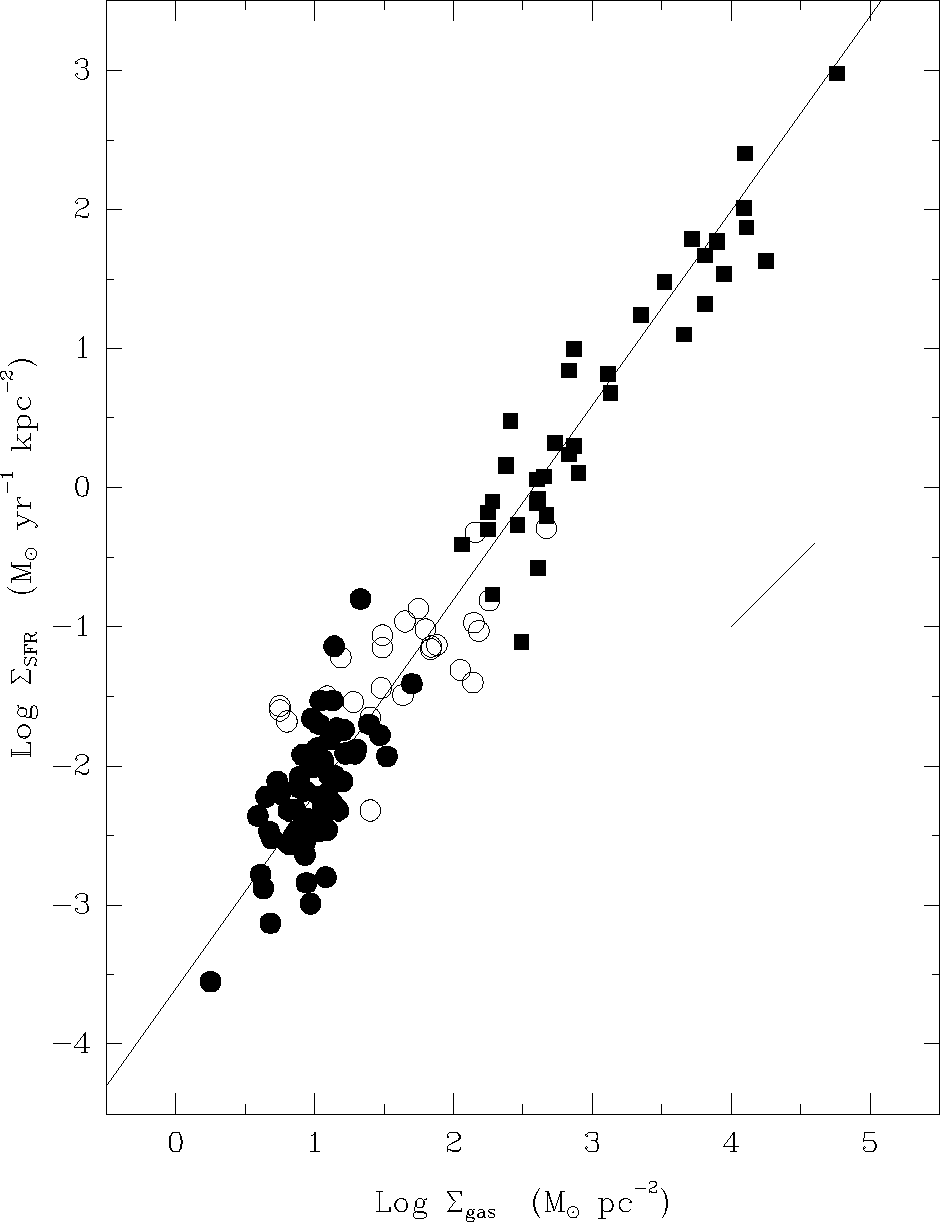
\includegraphics[width=0.6\textwidth]{graphics/gce/schmidt_kennicutt}
    \caption{The \ac{sfr} as measured by \citet{kennicutt98}. The continous line represents the best fit to the observations. \citet{kennicutt98}, \copyright\ 1998 The American Astronomical Society.}
    \label{fig:gce:schmidt_kennicutt}
\end{figure}
Figure~\ref{fig:gce:schmidt_kennicutt} shows the \ac{sfr} derived by \citet{kennicutt98}. The solid line represent the best fit to the shown observations and agrees with a $k=1.4\pm0.5$ in equation~\eqref{eqn:gce:schmidt_kennicutt_law}. The short, diagonal line represents the same scaling law with a change in scaling factor by a factor of two.

The initial mass function can also be derived from observations and has been previously shown in Figure~\ref{fig:star_formation:imf}. While the \ac{imf} is usually assumed to be constant in time, the \ac{sfr} varies depending on how much material is available for star formation. Using observations, \citet{scalo86} showed that the \ac{sfr} in the solar vicinity did not change by more than a factor of two during the disk lifetime. This represents an important constraint for \ac{gce} models.


\morebox{Observing the \ac{sfr}}{Proxy observations serve as the mechanism to determine the \ac{sfr} in the galaxy. Two examples of such observations are:
\begin{itemize}
    \item Observing supergiants, which have a short lifetime, under the assumption that their number is proportional to the \ac{sfr}. Note that these stars are so luminous that they can also be observed in other galaxies.
    \item Measure the H$_\alpha$ and $H_\beta$ flux from ionizied hydrogen (HII) regions. These regions are ionized by young and hot stars. Assuming that the flux from these stars is proportional to the \ac{sfr} leads to to the \ac{sfr} itself.
\end{itemize}
Other possibilites exist to measure the \ac{sfr}, see, e.g,. \citet{matteucci12}.}


\subsection{Stellar Yields}

Another important ingredient for \ac{gce} models are the stellar yields. A first distinction has to be made for potential stellar yields depending on the mass of the star. The lowest mass stars are brown dwarfs with masses $M<0.1\,M_\odot$. They never ignite hydrogen burning and do not enrich the \ac{ism} with elements. They therefore only lock up gas. Low mass stars furthermore have very long half-lives, e.g., around 10\,Ga for a star with mass $M_\odot$. This significantly limits their contributions to \ac{gce} and these stars therefore mainly lock up gas for the time being. 

Intermediate mass stars with masses $\lesssim 8\,M_\odot$ (Chapter~\ref{ch:sun}) form some $\alpha$ elements and are the hosts of the \ac{sproc}. These stars leave behind a planetary nebula at the end of their life and a \ac{wd}. Material in the \ac{wd} is locked up, however, the planetary nebula represents material that is effectively recycled back into the galaxy. 

Massive stars in the mass range between $8-10\,M_\odot$ likely explode as \acp{ecsn}, however, details on the exact mechanisms are still vague. Heavier stars with masses up to around $25\,M_\odot$ explode as regular core-collapse \acp{sn}. The explosion in both types releases a significant amount of $\alpha$ and iron peak elements. Furthermore, massive stars host the weak \ac{sproc} and might contribute to the formation of the \textit{p}-nuclei and maybe even host some form of the \ac{rproc}. It is unclear if heavier stars with masses $\gtrsim 25\,M_\odot$ undergo a \ac{sn} explosion or directly collapse into a \ac{bh}. However, they still can recycle a massive amount of elements by strong stellar winds, e.g., during their \ac{wr} phase.

\acp{snia} are expected to significantly contribute material to the galaxy, especially around the iron peak and maybe also some part of the \textit{p}-nuclei, which they could form in the $\gamma$-process. The exact scenario under which \acp{snia} take place is still a mystery, which also limits our current understanding of the exact nucleosynthesis processes that might take place. Importantly, no matter which scenario results in \acp{snia}, two stars have to first evolve fully in order to form one or two \acp{wd}. This scenario, as well as all merger scenarios, require time. Therefore, these element factories cannot contribute at the very beginning.

Finally, more contributors have been discussed before, e.g., classical novae (Chapter~\ref{ch:novae}). Furthermore, we have briefly mentioned super massive objects that could have formed at zero metallicity, see Chapter~\ref{sec:star_formation}. The nucleosynthesis yield of these stars still contain many uncertainties, are however important to consider \ac{gce} in the early Milky Way.

\subsection{Gas Flows}

\ac{gce} models that do not consider gas in- or outflow are called closed box models. Gas flows however into the galaxy from the metal-poor halo. Since this material has not been effectively processes through \ac{gce}, the inflowing gas is often assumed to be primordial. Gas infalling onto the disk is expected to transfer angular momentum to the gas in the disk, which induces radial flows of gas in the disk. 

Gas outflows are likely fundamental in the evolution of galaxies and have been observed in dwarf irregular starburst galaxies. The main cause for gas outflow from a galaxy are \acp{sn}, which accelerate the gas such that it can effectively be transported away from the galaxy. If the gas in fact leaves the gravitational well of the galaxy, it is called a galactic wind. If the gas however simply falls back onto the galaxy itself one speaks of a so-called galactic fountain.


\section{Models of Galactic Chemical Evolution}

\subsection{One-Zone Model}

One of the simplest models for \ac{gce} is the so-called one-zone model. Here, instantaneous mixing is assumed, which means that material released from stars is immediately recycled back into the galaxy. The Sun rotates around the center of the Milky Way with a period of around 240\,Ma. This timescale is rather fast compared to the age of the Milky Way, therefore instantaneous mixing is a good first-order assumption for a simple \ac{gce} model. For the one-zone model, we can write the evolution of metal $Z$ with respect to time as
\begin{equation}
    \frac{d(Zf_g)}{dt} = \underbrace{E_\mathrm{SW} + E_\mathrm{CCSN} + E_\mathrm{SNIa} + E_\mathrm{NSM}}_{\mathrm{Stellar\  Ejections}} - \underbrace{Z\psi}_{\mathrm{SFR}} + \underbrace{Z_\mathrm{in} R_\mathrm{in} - Z R_\mathrm{out}}_{\mathrm{Gas\ Flows}}.
\end{equation}
Here, $f_g$ is the fraction of material that is in gas form and thus available for star formation. The stellar ejection of metals is roughly composed of stellar winds ($E_\mathrm{SW}$), \acp{ccsn} ($E_\mathrm{CCSN}$), \acp{snia} ($E_\mathrm{SNIa}$), \ac{ns}-\ac{ns} merger ($E_\mathrm{NSM}$) contributions. Other sources, e.g., novae, have to be considered as well, however are of less importance. Once matter gets used up by star formation and therefore gets trapped for some amount of time, the star formation rate decreases, which is indicated by $-Z\psi$. Finally, gas inflow ($R_\mathrm{in}$) and outflow ($R_\mathrm{out}$) rates for given metals have to be considered. Note here that the inflowing matter does not necessarily have the same metallicity as the present one, i.e., $Z_\mathrm{in} \neq Z$.

\begin{figure}[tb]
    \centering
    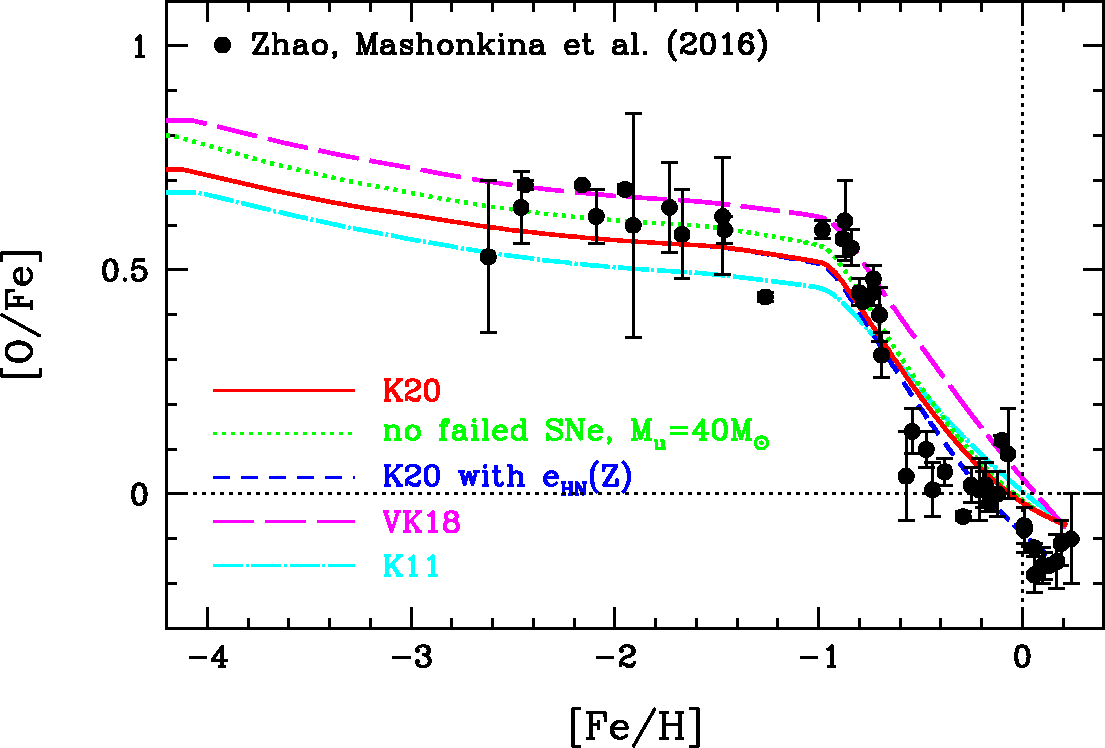
\includegraphics[width=0.65\textwidth]{graphics/gce/kobayashi20_fig3}
    \caption{Observations of the [O/Fe] ratio as a function of the [Fe/H] ratio in comparison with various \ac{gce} models. From \citet{kobayashi20}, , \copyright\ 2020 The American Astronomical Society.}
    \label{fig:gce:kob20_o_fe_versu_fe_h}
\end{figure}
Figure~\ref{fig:gce:kob20_o_fe_versu_fe_h} shows the [O/Fe] ratio as a function of the [Fe/H] in the solar neighborhood. Plotted are observations by \citet{zhao16} in comparison with different \ac{gce} models. The figure was taken from \citet{kobayashi20}. These authors also presented the top three \ac{gce} models that the observations are compared with in Figure~\ref{fig:gce:kob20_o_fe_versu_fe_h}. At the very left side of the figures, population III stars are expected to form the first metals in the galaxy. Such stars have not been observed, therefore no data points exist. The first ultra metal-poor stars that have been observed show up at an [Fe/H] of around -2.6. At this point in the \ac{gce} model, population II stars also form and start contributing. Note that for classic \ac{gce} models, especially the ones that assume instantaneous recycling, increasing [Fe/H] values on the horizontal axis correlate to the growing age of the galaxy. The kink in the observation and the model curve manifests the start of contributions by \acp{snia}. These \acp{sn} cannot contribute to the galaxy early on since they require a significant amount of time in order to develop low mass main sequence stars into \acp{wd}, then have to accrete mass (single degenerate scenario) or merge (double degenerate scenario) in order to produce a \ac{snia}. The [O/Fe] vertical axis in Figure~\ref{fig:gce:kob20_o_fe_versu_fe_h} is also correlated with age, however, not as straight forward as the horizontal axis. On top, \acp{ccsn} mainly contribute to the nucleosynthesis. Especially massive population III stars are expected to contribute a significant amount of oxygen to the galaxy. \acp{snia} on the other hand, which contribute only in the bottom right, are clearly the main producers of iron in the Milky Way. Once \acp{snia} start contributing, the abundance of iron significantly increases.

The red curve in Figure~\ref{fig:gce:kob20_o_fe_versu_fe_h} considers the single degenerate scenario for \acp{snia}. Interestingly, even with a mix of 75\% single degenerate, 25\% double degenerate \acp{snia} cases, the observations still agree. However, if only merging \acp{wd} cases are used for the \acp{snia} scenario, the kink shown in the observations flattens out. \ac{gce} models therefore allow us to determine that the majority of \acp{snia} must have the single degenerate scenario as their origin.

\begin{figure}[tb]
    \centering
    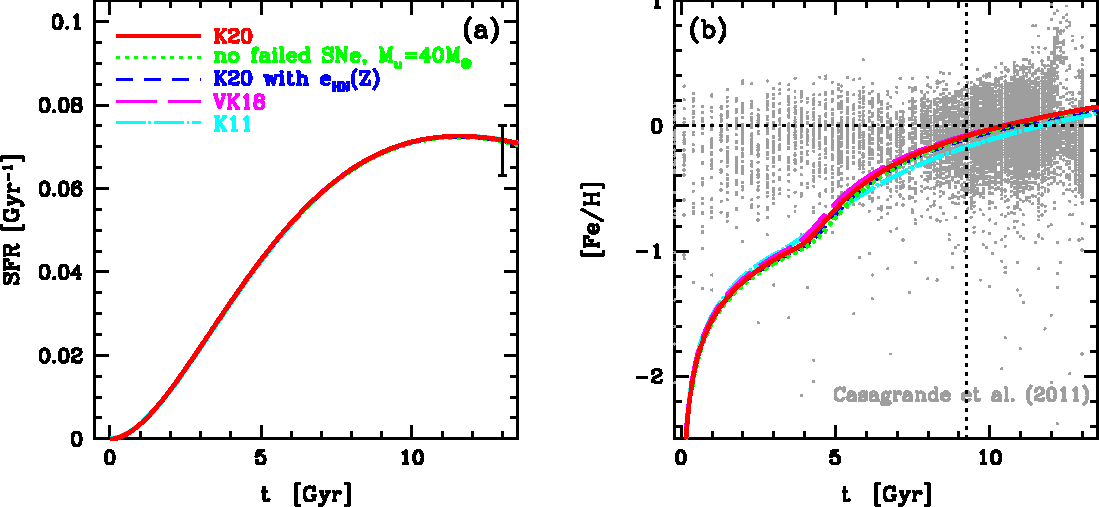
\includegraphics[width=\textwidth]{graphics/gce/kobayashi20_fig1ab}
    \caption{The \ac{sfr} (a) and [Fe/H] (b) evolution as functions of the age of the Milky Way. From \citet{kobayashi20}, \copyright\ 2020 The American Astronomical Society.}
    \label{fig:gce:kob20_sfr_and_fe_h_versus_time}
\end{figure}
In one-zone models, the \ac{sfr} and the [Fe/H] can be directly associated with the time the galaxy has evolved. These correlations are model dependent and are shown for the \ac{gce} model by \citet{kobayashi20} in Figure~\ref{fig:gce:kob20_sfr_and_fe_h_versus_time}. Observations by \citet{casagrande11} however show that these simple evolution cannot explain the totality of the observed spread. 

While one-zone chemical evolution models are simple and neglect many details, they still allow us to draw important conclusions, e.g., which scenario is likely the origin of \acp{snia}. These models also allow us to track the evolution of all elements in a self-consistent way. Details for the model by \citet{kobayashi20} are discussed later in Section~\ref{sec:gce:chemical_evolution_solar_neighborhood}.


\subsection{Chemodynamical Models}

Chemodynamical models follow the evolution of a galaxy from the Big Bang to today's composition. Individual nucleosynthesis events are modeled using so-called star particles. These star particles are allowed to orbit the galaxy and are tracked. Ejecta from a given star particle is not instantaneously available in the whole galaxy, but mixing is calculated using a hydrodynamice prescription of the gas within the framework of the the \ac{gce} model. 

\begin{figure}[tb]
    \centering
    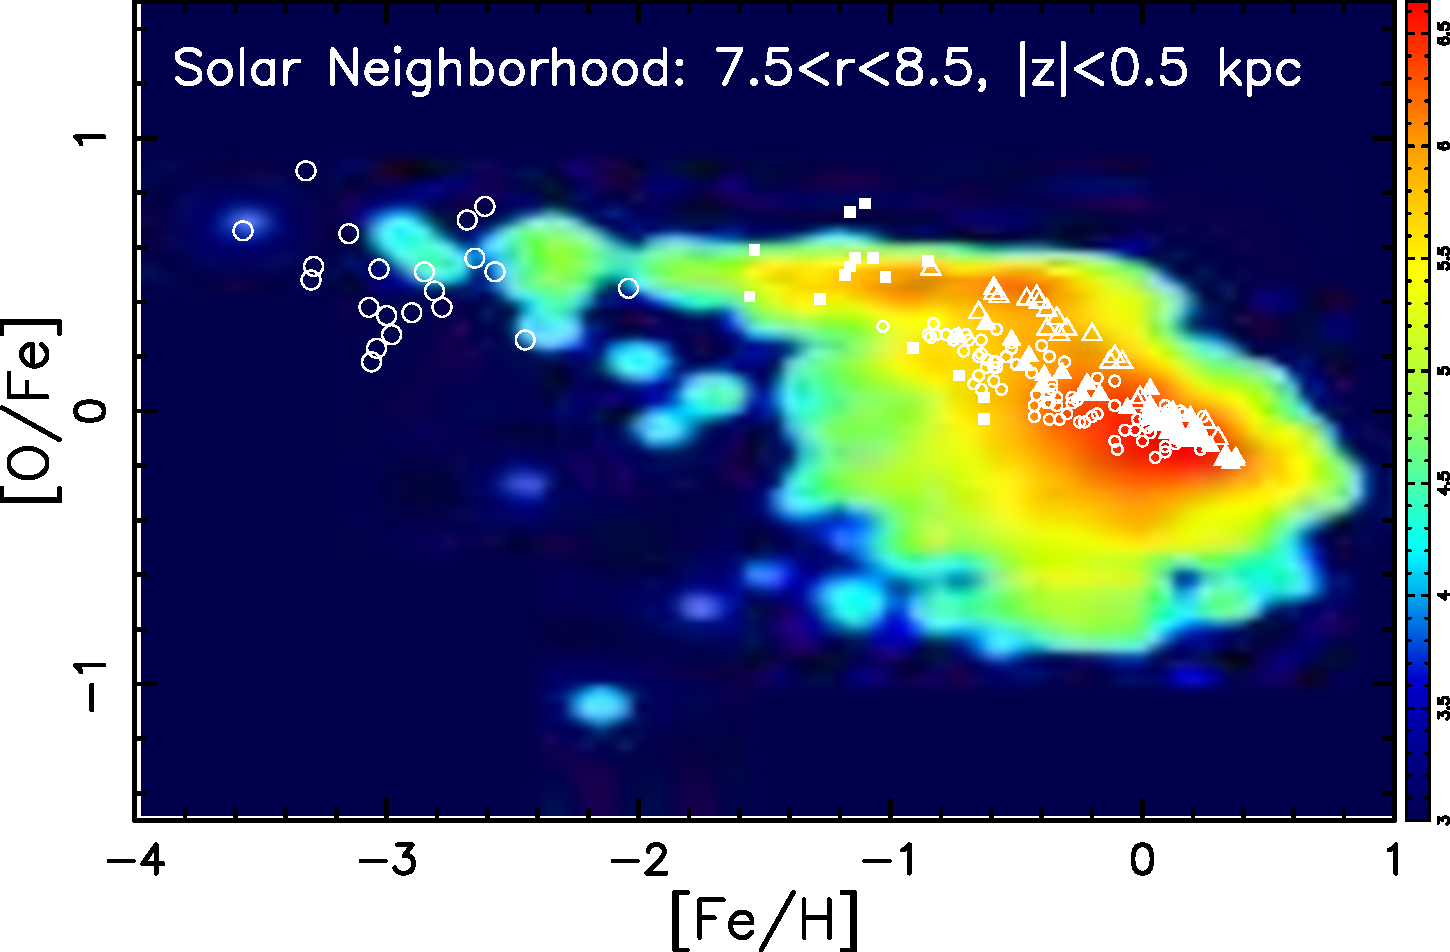
\includegraphics[width=0.65\textwidth]{graphics/gce/kobayashi11_fig10a}
    \caption{Observations of the [O/Fe] ratio as a function of the [Fe/H] ratio in comparison with a chemodynamical model for the solar neighborhood. From \citet{kobayashi11}, \copyright\ 2011 The American Astronomical Society.}
    \label{fig:gce:kob11_o_fe_versus_fe_h}
\end{figure}
Figure~\ref{fig:gce:kob11_o_fe_versus_fe_h} shows observations of [O/Fe] as a function of [Fe/H] for the solar neighborhood in comparison with the chemodynamical model of \citet{kobayashi11}. This figure is analog to Figure~\ref{fig:gce:kob20_o_fe_versu_fe_h}. The colors indicate the frequency distribution of model predictions. Clearly, chemodynamical models can track the heterogeneous evolution of the Milky Way since instantaneous recycling is not required. However, these models are also computationally more expensive and thus have limitations in how many species can be tracked.


\subsection{The Impact of Assumptions and Uncertainties}

Since one-zone models are computationally simple, they can be used in combination with \acf{mcmc} methods\footnote{See, e.g., \href{https://en.wikipedia.org/wiki/Markov_chain_Monte_Carlo}{Wikipedia} for more details.} to study the effect of model assumptions and uncertainties, e.g., in the nuclear physics parameters. An interesting study was recently presented by \citet{cote17}. 
\begin{figure}[tb]
    \centering
    \includegraphics[width=0.75\textwidth]{graphics/gce/sculptor}
    \caption{The Sculptor Galaxy 13 million light years away from the Earth. Credit: \href{https://www.eso.org/public/images/eso1025a/}{ESO/J. Emerson/VISTA}. Acknowledgment: Cambridge Astronomical Survey Unit.}
    \label{fig:gce:sculptor}
\end{figure}
These authors presented simple one-zone \ac{gce} models for the Sculptor galaxy (Figure~\ref{fig:gce:sculptor}). Using \ac{mcmc} they determined the best set of input parameters to a one-zone model when modeling the evolution of nine different elements. These models show that success or failure for a \ac{gce} model in reproducing an observed galaxy mainly depends on the stellar yields that are used. Simple, one-zone models thus can significantly constrain \ac{gce} and help to constrain the stellar yields and their applicability.

\codebox{NuPyCEE}{The NuGrid collaboration publishes the \acf{nupycee} as open source code. Here, easy-to-read python code, documentation, and user guides are published. This allows users to simulate the chemical enrichment and stellar feedback of stellar populations. These codes were, e.g., used in \citet{cote17}. Details can be found on the website at \url{http://nugrid.github.io/NuPyCEE/}.}



\section{Chemical Evolution of the Solar Neighborhood} \label{sec:gce:chemical_evolution_solar_neighborhood}

\citet{kobayashi20} recently modeled the evolution of the solar neighborhood. Figure~\ref{fig:gce:kob20_o_fe_versu_fe_h} already showed the [O/Fe] as a function of the [Fe/H], which can be used to constrain the scenario responsible for the majority of \acp{snia} as discussed above. The evolution of most elements can be constrained well with spectroscopic observations. Let us first discuss the origin of neutron capture elements beyond the iron peak in the solar neighborhood. These elements and their isotopes mainly formed in the \ac{sproc} and \ac{rproc}. \ac{gce} models allow us to study the likely sources of these neutron capture elements, especially for the \ac{rproc} for which the nucleosynthetic sources are so-far unclear (see Chapter~\ref{ch:r-process}).

\begin{figure}[tb]
    \centering
    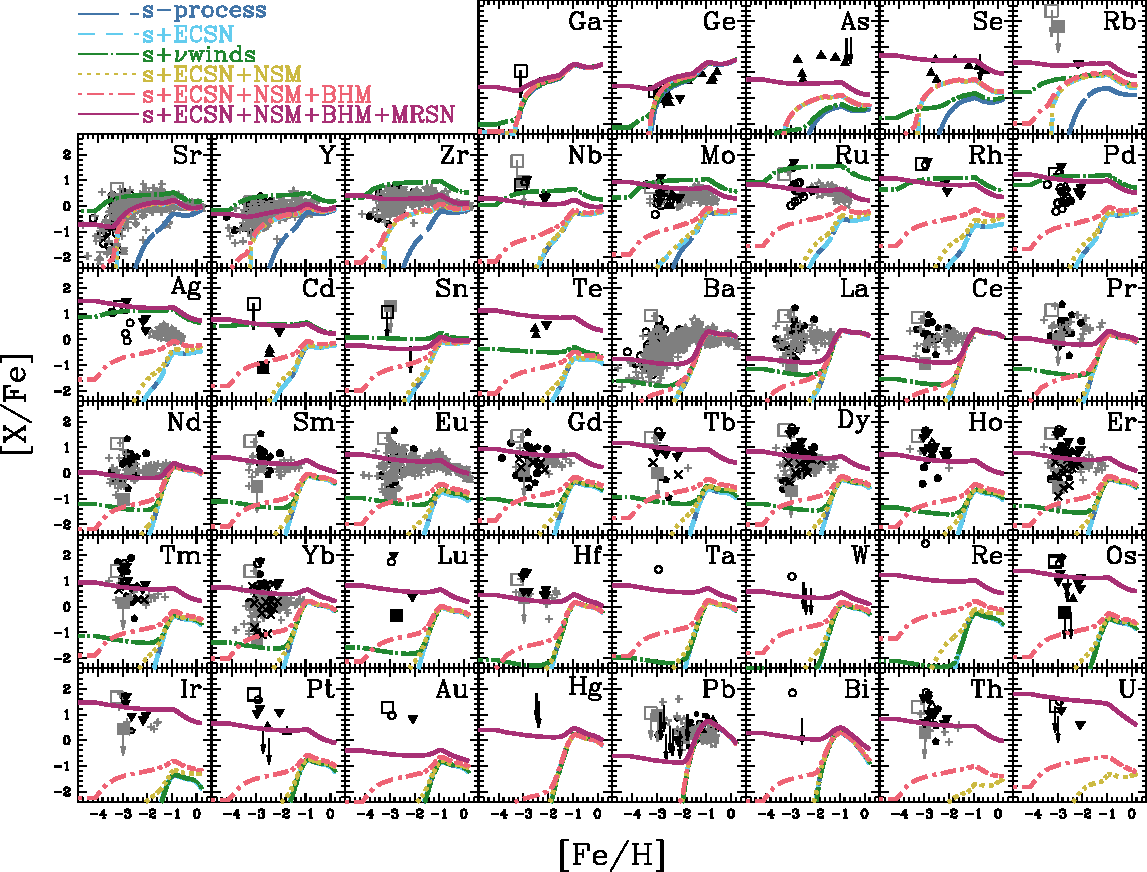
\includegraphics[width=\textwidth]{graphics/gce/kobayashi20_fig32}
    \caption{The evolution of neutron capture elemental abundnaces in the solar neighborhood. The various sources are discussed in the text. From \citet{kobayashi20}, \copyright\ 2020 The American Astronomical Society.}
    \label{fig:gce_kob20_element_evolution_various_processes}
\end{figure}
Figure~\ref{fig:gce_kob20_element_evolution_various_processes} shows the evolution of the neutron capture elements in the solar neighborhood as modeled by \citet{kobayashi20}. The vertical axis of each plot is the [X/Fe] ratio, where X is the element that is plotted and noted in each sub-window. The evolution of all these elements are plotted as a function of [Fe/H]. The dark-blue curve shows only contributions by the \ac{sproc} in \ac{agb} stars. Clearly, the main \ac{sproc} cannot explain the composition of most neutron capture elements, except for today's amount of some elements such as barium, lanthanum, cerium, and lead. Adding only yields of \acp{ecsn} to the existing model changes almost none of the abundances, except for the light \ac{sproc} elements such as strontium and zirconium. Adding neutrino-driven winds, see the green curve labeled ``s + $\nu$winds'', shows a significant effect for the light elements and in fact even overproduces most of them. Therefore, neutrino-driven winds are generally left out of \ac{gce} because their yields seem to be too high at the moment. 

Further combinations of various stellar yields are the combination of \ac{sproc}, \acp{ecsn} and \ac{ns}-\ac{ns} mergers (denoted ``NSM''), shown in beige. This addition adds some heavy \ac{rproc} nuclei, however, does not seem to produce enough material in order to explain the observations of, e.g., the actinides. The rates get slightly higher when including as well \ac{ns}-\ac{bh} mergers (pink curve), however, still not enough \ac{rproc} nuclei are produced. In Section~\ref{sec:r-process:open_questions:europium_problem} we already discussed that very high levels of europium have been detected in metal-poor stars. This can also be seen in Figure~\ref{fig:gce_kob20_element_evolution_various_processes}. In the framework of \citet{kobayashi20}, this europium problem cannot be solved by \ac{ns}-\ac{ns} or \ac{ns}-\ac{bh} mergers. Thus, additional \ac{rproc} sources are required to explain these observations.

In order to explain the abundances of all neutron capture elements including the clear \ac{rproc} indicators, \citet{kobayashi20} included stellar yields from \acf{mhdjsn} models, see Section~\ref{sec:r-process:astrophysical_sites:supernovae}. These hypothetical models would add enough \ac{rproc} material to explain most of the observations, as can be seen when looking at the purple curve in Figure~\ref{fig:gce_kob20_element_evolution_various_processes}. Some elements, e.g., gold, are still underproduced even when including all these sources. However, gold is an especially difficult element to observationally constrain and only a very limited amount of data is currently available. 

Note that the contributions of \ac{ns}-\ac{ns} or \ac{ns}-\ac{bh} mergers is highly dependent on the adopted rate of these events. This rate is currently associated with large uncertainties, however, will improve over time as \ac{ligo} detects more and more of these events. Therefore, the final word on which events contribute the \ac{rproc} elements in the right amounts is surely not yet spoken.

\begin{figure}[tb]
    \centering
    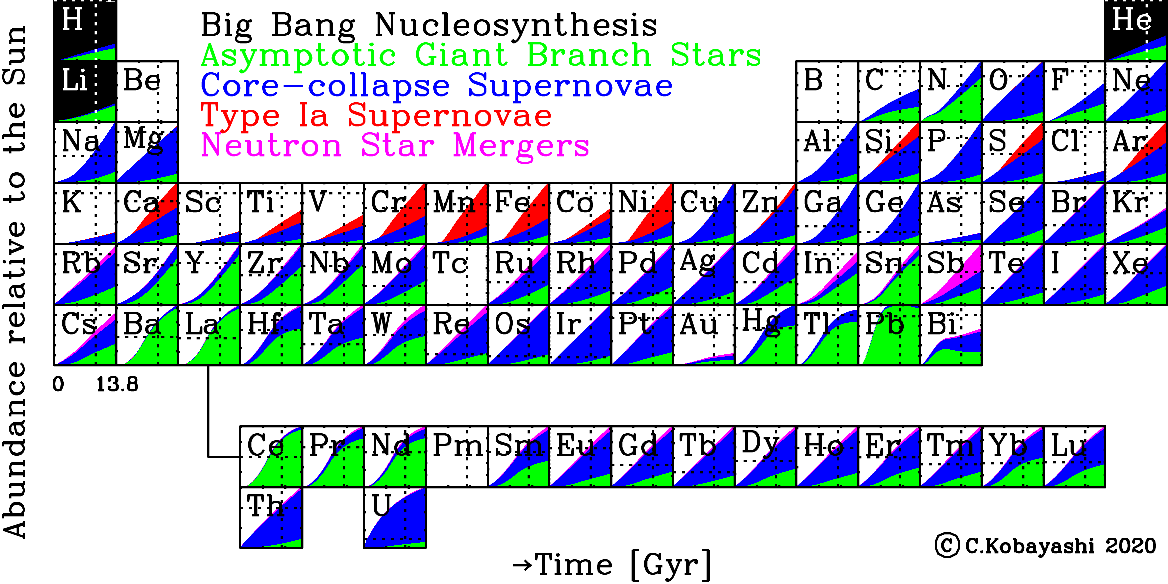
\includegraphics[width=0.9\textwidth]{graphics/gce/kobayashi20_fig39}
    \caption{Time evolution of all elements in the solar neighborhood over the lifetime of the Milky Way. The cross indicates the solar composition at its start 4.567\,Ga ago. From \citet{kobayashi20}, \copyright\ C. Kobayashi 2020 / 2020 The American Astronomical Society.}
    \label{fig:gce:kob20_origin_elements}
\end{figure}
Figure~\ref{fig:gce:kob20_origin_elements} shows the evolution of all elements displayed in the form of the periodic table. The horizontal axis of each square goes from the beginning of the Milky Way to its current age of 13.8\,Ga. The solar composition at its beginning 4.567\,Ga ago is shown as a dotted cross. The different stars that contribute elements are shown in color. Note that this figure is not equivalent to Figure~\ref{fig:gce_kob20_element_evolution_various_processes}. Here, the various stars that contribute to each element are shown and not the processes that formed the elements in the first place. For example, Figure~\ref{fig:gce:kob20_origin_elements} shows that part of the uranium and thorium is ejected and recycled by \ac{agb} stars. While actinides cannot form in the \ac{sproc}, most \ac{agb} stars started off with some metals, i.e., as population II or I stars. They therefore simply keep their original actinide composition and recycle it back into the Milky Way when they die.


\section{Reading}

The motivated reader is highly encouraged to read the original work by \citet{kobayashi20}, which was heavily used in this chapter as an excellent example of \ac{gce}. 
On October 2, 2020, Chiaki Kobayashi also gave a talk for the \acf{irena} seminar. This talk was recorded and is available on the web.\footnote{\url{https://youtu.be/GZcVGueXKp0}}

For this week's chapter, we will read and discuss \citet{cote21}, who modeled the \ex{129}I and \ex{247}Cm isotope ratio and compared it with the known early solar system value. This work also serves as an excellent introduction to the next chapter. Some discussion points that might help you with the reading are summarized below:
\begin{itemize}
    \item What makes \ex{129}I and \ex{247}Cm ideal nuclei to study the sources that produced these isotopes before the Solar System formed?
    \item How is \ac{gce} modeled in this work and why?
    \item How do the different scenarios of \ac{ns}-\ac{ns} merger ejecta compare to each other? What are the conclusions for \ac{mhdjsn} models?
    \item What does this work tell us about the origin of the \ac{rproc} elements in the Milky Way?
\end{itemize}